\documentclass[main.tex]{subfiles}

\begin{document}

\section{Offer Networks}
An \textbf{offer network} instance can be formally modeled as a directed graph where vertices $t \in T$ represent tasks and labeled directed edges $(t_a,t_b) : u_1$ represent an offer by user $u_1$ to do task $t_a$ in exchange requested task $t_b$.
\begin{center}
  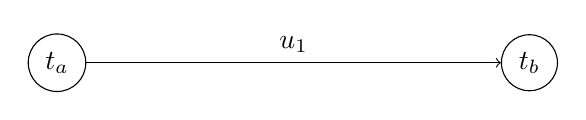
\begin{tikzpicture}
    \node[draw, circle] (ta) at (0,0) {$t_a$};
    \node[draw, circle] (tb) at (6,0) {$t_b$};
    \path [->] (ta) edge node[above] {$u_1$} (tb);
  \end{tikzpicture}
\end{center}

A matching of users who can satisfy each other is a vertex cycle. See the simplest case below:

\begin{center}
  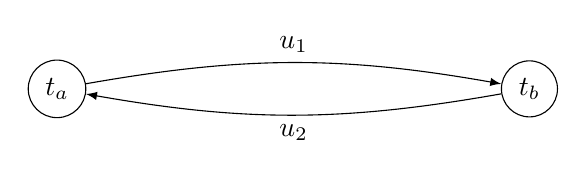
\begin{tikzpicture}
    \node[draw, circle] (ta) at (0,0) {$t_a$};
    \node[draw, circle] (tb) at (6,0) {$t_b$};
    \draw[-latex] (ta) to[bend left=10] node[above] {$u_1$} (tb);
    \draw[-latex] (tb) to[bend left=10] node[below] {$u_2$ }(ta);
  \end{tikzpicture}
\end{center}

The cycle packing problem \cite{Kri} characterises the goal of the matcher: find as many cycles with distinct edges (offer-request pairs). This problem is NP-Hard, although \cite{Kri} has an $\bO(\sqrt{\log n})$-approximation algorithm for it. I'm not yet clear whether the algorithm works with multiple edges between two nodes.

The matching problem can also be stated in terms of Weighted Boolean Optimization, a form of Integer Programming. Some additional features may be easier to add in this case, which is a common, reliable choice in the field despite being NP-complete.

Below is a list of potentially desirable features that don't qualify for an MVP\footnote{minimal viable prototype}:
\begin{itemize}
  \item Reputation biased matching
  \item Preferences for matching based on
    \begin{itemize}
      \item User preferences
      \item Task prefreences
    \end{itemize}
  \item ORs and ANDs of offers or request
\end{itemize}


\end{document}
